\section{Voltage Supplies}\label{sec:voltage-supplies}

	\subsection{Power Supplies}\label{ssec:power-supplies}
		In order to avoid any interference of the AC line, this project will work with a DC voltage input and any other necessary voltages will be acquainted from this higher input voltage supply.There are many different types of voltage regulators, nowadays the most common DC/DC being switching regulators. They are more efficient than linear regulators and consequently they waste less heat, the downside is the cost (due their consequently) and that they tend to have some ripple at the output \cite{schweber2017}. However, as this project does not aim radical cost management and as this ripple can be filtered, this type of voltage regulator was choosen for this project.

		\subsubsection{5V Supply}\label{sssec:5v-supply}
			Most of the choosen components for this project were choosen so they would be capable to work with single-supply of 5V. The choosen voltage regulator for the 5V supply was the TL2575-05 from \textit{Texas Instruments} \cite{tl2575-05-datasheet}, it has a output up to 1A, voltage drop ov 2V and typical efficiency of 88$\%$. Figure \ref{fig:tl2575-05-circuit} shows the circuit used for the 5V supply.

			\begin{figure}[htbp]
				\centering
					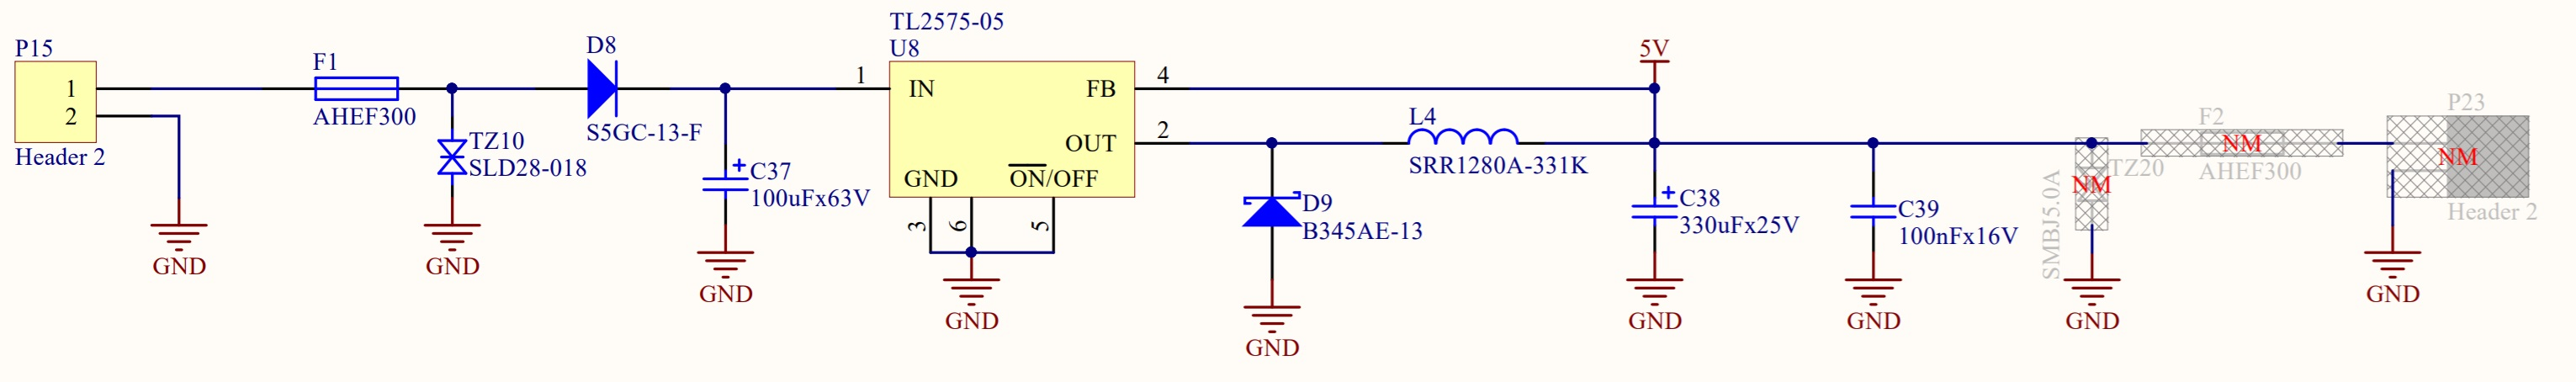
\includegraphics[scale=1.5]{figuras/fig-tl2575-05-circuit.png}
				\caption{5V Power Supply Circuit \cite{tl2575-05-circuit}}
				\label{fig:tl2575-05-circuit}
			\end{figure}

			The diode FM205-W from \textit{Rectron Semiconductor} \cite{fm205-2-datasheet} is used to protect the input of converter from inverse polarity. This diode has a maximum current of 2A, twice the maximum curret output of the regulator, so it will not interfere with the input current. Inductor L4 is fundamental for the device to work according to the datasheet. Capacitors C16 and C17 are a bypass capacitors recommended by the converter's datasheet. Diode D3 is a catch diode used to protect the converter from flyback currents from the inductor, the datasheet only specifies it should be a Schottky diode with maximum current at least the same as the maximum output current of the converter (1A). The choosen diode is FM5819-W from \textit{Rectron Semiconductor} \cite{fm5819-w-datasheet}.
			\par
			According to the datasheet this circuit has a input voltage from 7V to 40V.
\begin{comment}
		\subsubsection{12V Supply}\label{sssec:12v-supply}
			For the 12V supply the choosen regulator was LM2574-12 from \textit{Texas Instruments} \cite{lm2574-12-datasheet}, it has a output up to 500mA, voltage drop of 2V, and typical efficiency of $88\%$. Figure \ref{fig:lm2574-12-circuit} shows the circuit used for the 12V supply.

			\begin{figure}[htbp]
				\centering
					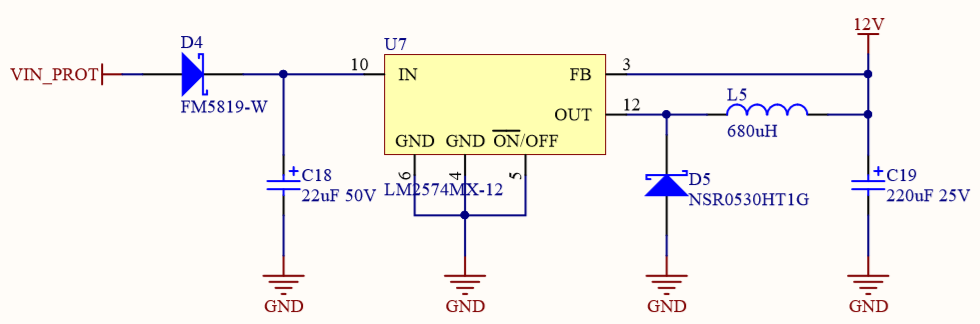
\includegraphics[scale=1.8]{figuras/fig-lm2574-12-circuit.png}
				\caption{12V Power Supply Circuit\cite{lm2574-12-circuit}}
				\label{fig:lm2574-12-circuit}
			\end{figure}	

			The diode FM5819-W from \textit{Rectron Semiconductor} \cite{fm5819-w-datasheet} is used to protect the input of converter from inverse polarity. This diode has a maximum current of 1A, twice the maximum curret output of the regulator, so it will not interfere with the input current. Inductor L5 is fundamental for the device to work according to the datasheet. Capacitors C18 and C19 are a bypass capacitors recommended by the converter's datasheet. Diode D5 is a catch diode used to protect the converter from flyback currents from the inductor, the datasheet only specifies it should be a Schottky diode with maximum current at least the same as the maximum output current of the converter (0.5A). The choosen diode is NSR0530HT1G from \textit{ON Semiconductor} \cite{NSR0530HT1G-datasheet}.
			\par
			According to the datasheet, this circuit has a input voltage from 14V to 40V.	
\end{comment}
		\subsubsection{Voltage Input Protection}\label{sssec:voltage-input-protection}

			Figure \ref{fig:input-protection-circuit} show the circuit used to protect the power supplies.

			\begin{figure}[htbp]
				\centering
					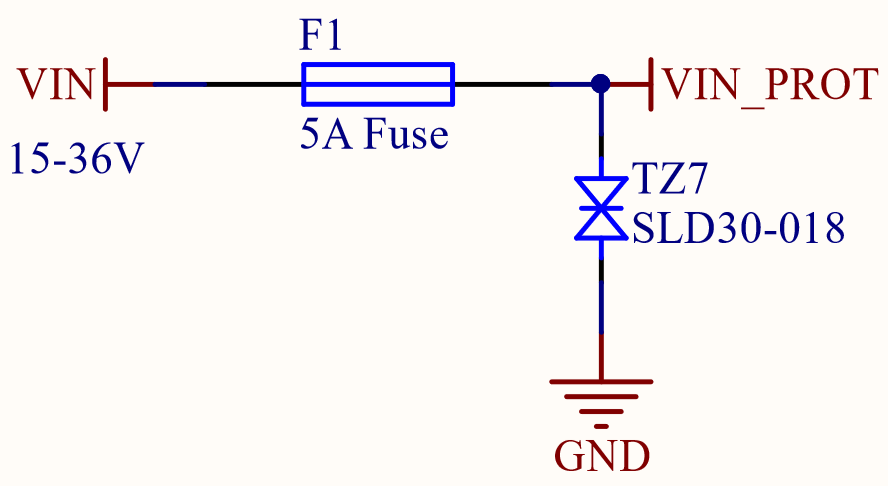
\includegraphics[scale=1]{figuras/fig-input-protection-circuit.png}
				\caption{Voltage Input Protection Circuit \cite{input-protection-circuit}}
				\label{fig:input-protection-circuit}
			\end{figure}

			TZ7 is a TVS diode used to protect the circuit against overvoltages. The choosen TVS is the SLD24-018, it has a standoff voltage of 24V and a maximum clamping voltage of 38.9 volts (check Section \ref{ssssec:tvsSelection}). Using this TVS limits the input voltage from 14-24V, in the other hand it ensures protection for the voltage regulators. D2 is a Schottky Diode used to protect the circuit against inverse polarity. The choosen diode is the 1N5822 \cite{1n5822-datasheet} from Vishay, this diode has a continuous forward current of 3A, a peak surge current of 80A  with a 8.3ms response time, making it suitable for protecting the circuit against reverse polaity. During the circuit assembly a fuse should be placed between the connector and the board.
			
	\subsection{Voltage References}\label{ssec:voltage-references}

		In this project any power supply that the precision and stability of the output voltage is more concerning than the maximum output current will be called a voltage reference.

		\subsubsection{10V Reference}\label{sssec:10v-reference}
			As it was explained in Section \ref{ssec:load-cell-signal-conditioning}, this voltage reference will be used to excite the load cells sensors of this project. The choosen component for this reference was the LM78L10 from \textit{Microchip} \cite{LM78L10-datasheet}. According to the datasheet, this voltage reference has a typical tolerance of $\pm 0.2\%$ and has maximum operating output current of 100mA. Load cells have a typical bridge resitance from 350$\Omega$ to 1k$\Omega$ \cite{GMIloadcell}. It was defined on this project requirements on Item \ref{itm:func-req-9} in Section \ref{sec:functionalRequirements} that the system must have two brake pressure acquistion channels. Hence, having two load cels with 350$\Omega$ bridge resistance and 10V excitation, 68mA of current would be needed, 100mA from the voltage reference would be suitable. Figure \ref{fig:LM78L10-circuit} shows to reference circuit.

			\begin{figure}[htbp]
				\centering
					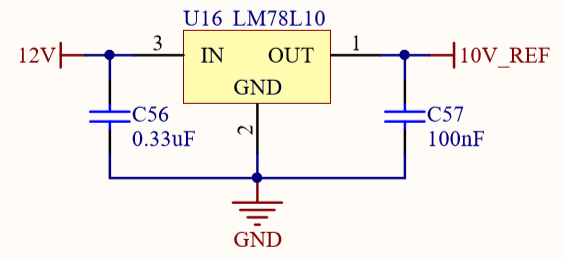
\includegraphics[scale=1.35]{figuras/fig-LM78L10-circuit.png}
				\caption{10V voltage reference circuit \cite{LM78L10-circuit}}
				\label{fig:LM78L10-circuit}
			\end{figure}

			The device's datasheet recommends using two decoupling capacitors, one in the input and other in the ouput with the given values from Figure \ref{fig:LM78L10-circuit}.

		\subsubsection{4V5 Reference}\label{sssec:4v5-reference}

			As said in Section \ref{ssec:thermocouple-sensor-detection}, the sensor detection circuit needs a 4V5 voltage reference for the comparator. This is achieved using the MAX6107EUR+T from \textit{Maxim Integrated} \cite{max6107eur+t-datasheet}. This is a precise 4V5 voltage reference and according to the datsheet it has a tolerance of $\pm0.4\%$ and a maximum operating output current of 5mA. Figure \ref{fig:max6107-circuit-circuit} shows the circuit for the 4V5 voltage reference.

			\begin{figure}[htbp]
				\centering
					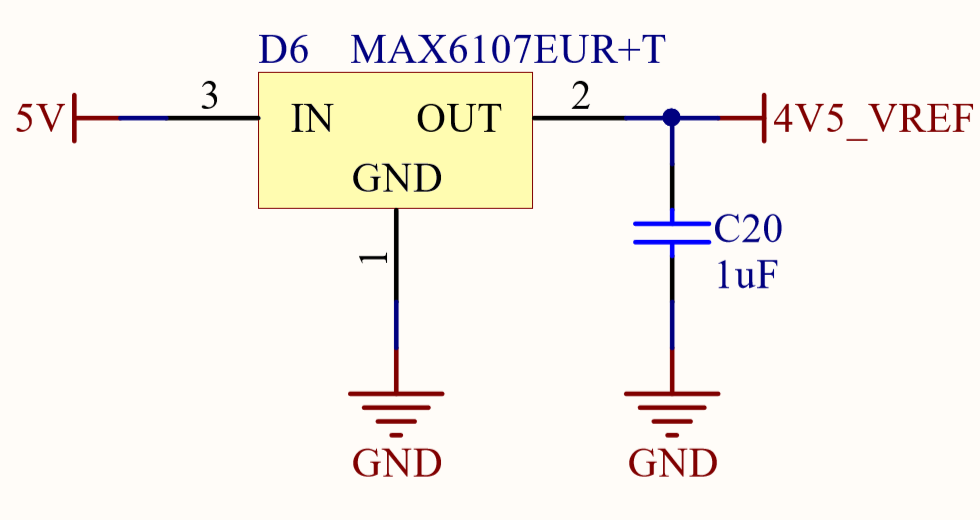
\includegraphics[scale=1.1]{figuras/fig-max6107-circuit.png}
				\caption{4V5 voltage reference circuit \cite{max6107-circuit-circuit}}
				\label{fig:max6107-circuit-circuit}
			\end{figure}

			According to the datasheet the only needed extra component is a decoupling capacitor at the output.

		\subsubsection{1V Reference}\label{sssec:1v-reference}

			The 1V reference from the circuit of Section \ref{ssec:ckp-signal-conditioning-circuit} is achieved using the ADR510ARTZ from \textit{Analog Devices} \cite{adr510artz-datasheet}. This is a 1V precision voltage reference with a tolerance of $\pm 0.35\%$ and maximum operating output current of 10mA. Figure \ref{fig:adr510-typical-circuit} shows the typical circuit using this voltage reference.

			\begin{figure}[htbp]
				\centering
					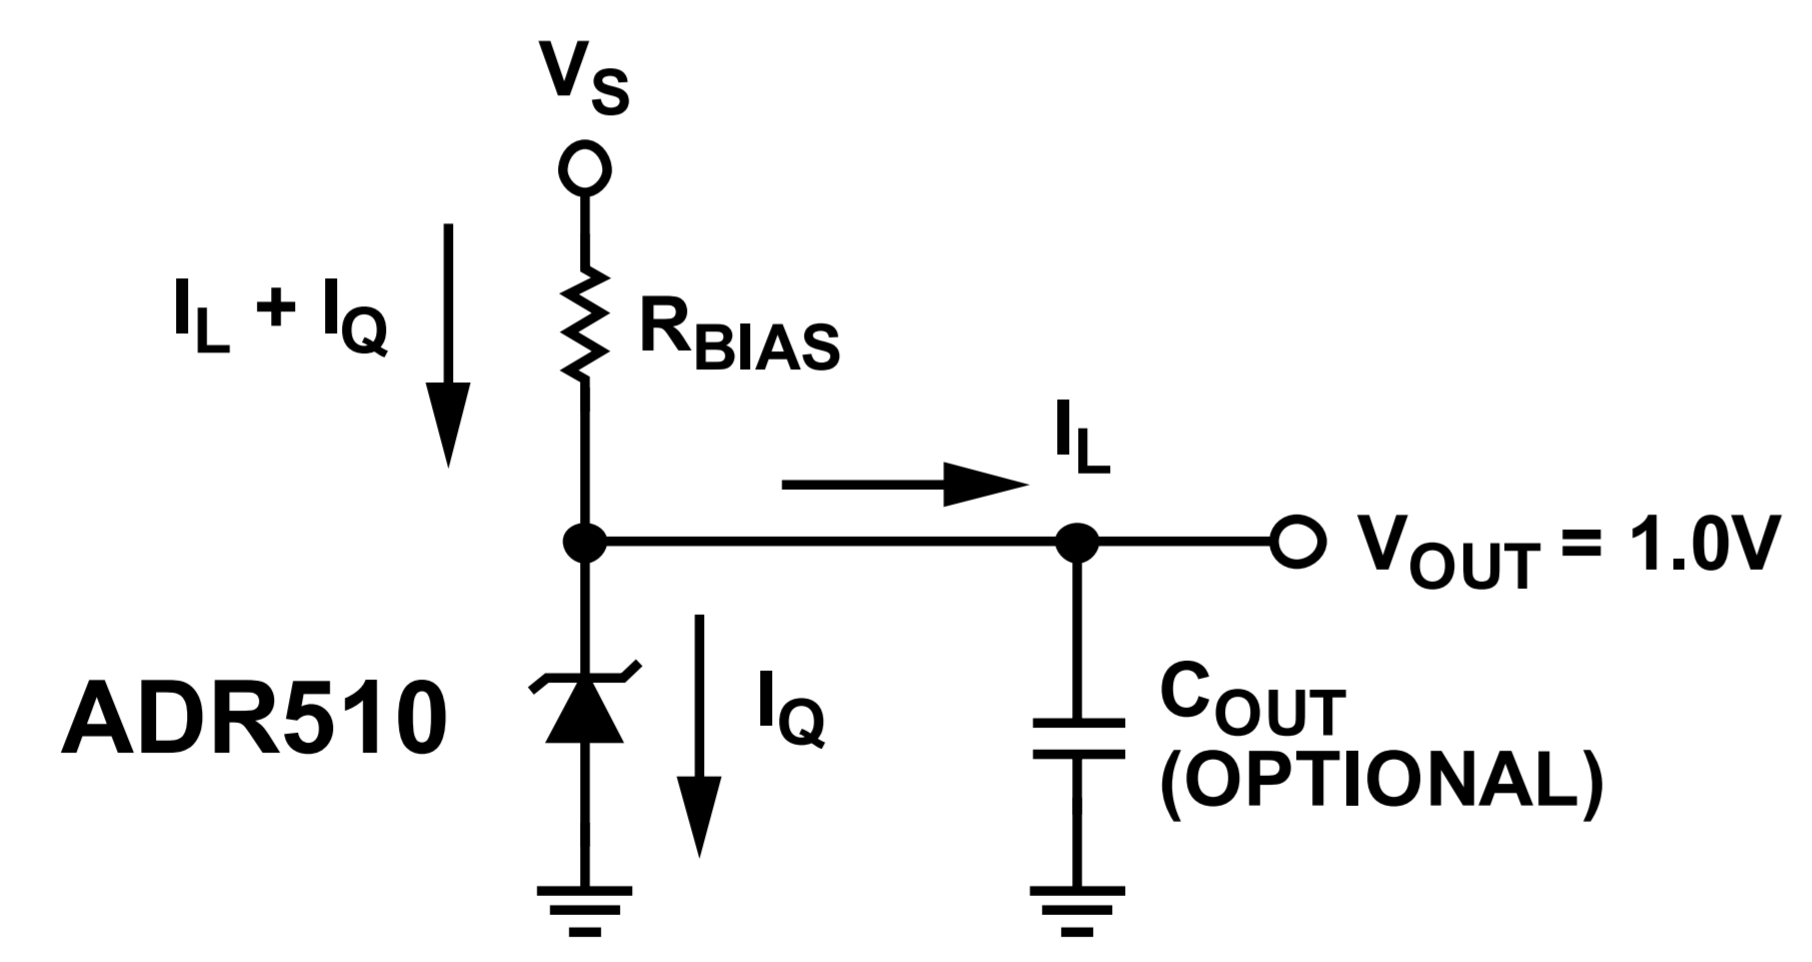
\includegraphics[scale=0.5]{figuras/fig-adr510-typical-circuit.png}
				\caption{ADR510 Typical Operating Circuit \cite{adr510-typical-circuit}}
				\label{fig:adr510-typical-circuit}
			\end{figure}

			The only external component needed is a bias resistor which can be calculated using \ref{eqn:rbis-adr510} \cite{adr510artz-datasheet}.

			\begin{equation}\label{eqn:rbis-adr510}
				R_{BIAS} = \frac{V_{S} - V_{OUT}}{I_{L} - I_{Q}}
			\end{equation}

			The used $V_{S}$ \textit{Voltage Supply} will be the 5V obtained in the circuit from Figure \ref{fig:tl2575-05-circuit} in Section \ref{sssec:5v-supply}. According to the datasheet, the minimul operating voltage ($I_{Q}$ in this case) is 100uA. Moreover, $V_{OUT}$ is naturally 1V5. The minimum bias current (load current $I_{L}$) is of 500nA (according to the IC that used the 1V reference \cite{lm2907-datasheet}). Hence, any value of resistance that guarantee that the current that flows through the regulator is less than 10mA is acceptable.
			\par
			Using a 1k$\omega$ resistor a current of 4mA can be achieved. Figure \ref{fig:ADR510ARTZ-circuit} shows the circuit for the 1V reference, the capacitor is just a decoupling capacitor recommended by the datasheet.

			\begin{figure}[htbp]
				\centering
					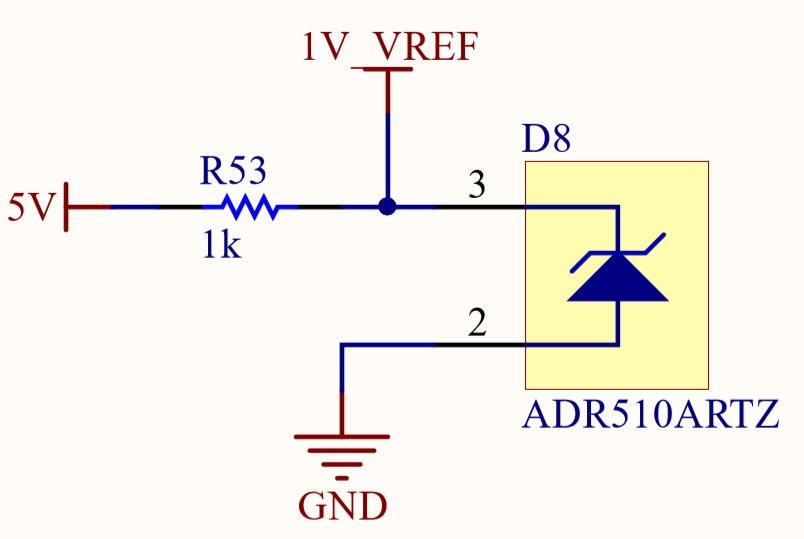
\includegraphics[scale=1.2]{figuras/fig-ADR510ARTZ-circuit.png}
				\caption{1V voltage reference circuit \cite{ADR510ARTZ-circuit}}
				\label{fig:ADR510ARTZ-circuit}
			\end{figure}	 

